\documentclass[11pt,a4paper,oneside]{article}
\renewcommand{\baselinestretch}{1.2}
\usepackage{sectsty,setspace,natbib,wasysym} 
\usepackage[top=1.00in, bottom=1.0in, left=1in, right=1.25in]{geometry} 
\usepackage{graphicx}
\usepackage{latexsym,amssymb,epsf} 
\usepackage{epstopdf}
\usepackage{amsmath}
\usepackage{hyperref}

%\graphicspath{{D:/Documents/Github/temporalvar/figures}{C:/Documents/Github/temporalvar/figures}}
\graphicspath{{../../figures/}}

\newenvironment{smitemize}{
\begin{itemize}
  \setlength{\itemsep}{1pt}
  \setlength{\parskip}{0pt}
  \setlength{\parsep}{0pt}}
{\end{itemize}
}

\usepackage{fancyhdr}
\pagestyle{fancy}
\fancyhead[LO]{December 2013}
\fancyhead[RO]{Variable environments \& climate change}

\begin{document}
\renewcommand{\labelitemi}{$-$}
\title{Coexistence and climate change: \\The role of
    temporal-variability in structuring future communities \\Updating To Do List from Skype Meetings}
    \author{Wolkovich \& Donahue}
\date{Last updated: 26 Aug 2014}
\maketitle

\newpage
\tableofcontents

\section{Skype Meeting - August 24, 2014}
\begin{itemize}
\item Running PhenologyModel.R does not produce coexistence even with two species set with the same parameters as Chesson et al 2004.  In Chesson et al 2004, species' biomasses bounce around 0.2.  Our sims drop to very low numbers by year 30.  Why?
\item Previous sims which stepped thru within year dynamics resulted in coexistence
\item Tried: decreasing extinction threshold to 1/100000 from 1/10000.  This does increase persistence (obviously) but does not change the pattern of species bouncing at very low densities
\item Tried: increasing the within-season time to 8 days from 5 days.  I did this because the in some years it wasn't clear from the plots (I did not check the numerics) that the species had reached max biomass.  Not clear that this had any effect.
\item Compared to Chesson: there are a few details of the simulation that aren't clearly laid out in Chesson et al 2004.  Particularly, it isn't clear when "flowering" occurs.  That is,  when is the end of the season?  we take the max biomass of each species, but could have a set flowering time for both species (say, when R<R*).  However, I think we have made a reasonable choice here and that, while it might result in differences with Chesson et al 2004, it should not result in the problem at hand.
\item Things to look at: what does R-uptake look like within a season?  Does it match the patters in Fig 2 of Chesson et al 2004?
\item: To do: when preparing for ASN, I changed the within-year simulation from a for-loop to an ode solver.  I did this because the within-season step size needed to be adjusted for differences in initial biomass and resource level: if step size was small enough to catch the crossing of the Rstar threshold, then it took forever the rest of the season.  However, I never completed the comparison of the ode solver and the within year for-loop.  That is the next task
\end{itemize}

\section{Megan: September 8 and  15, 2014}
\begin{figure}[h!]
\centering
\noindent 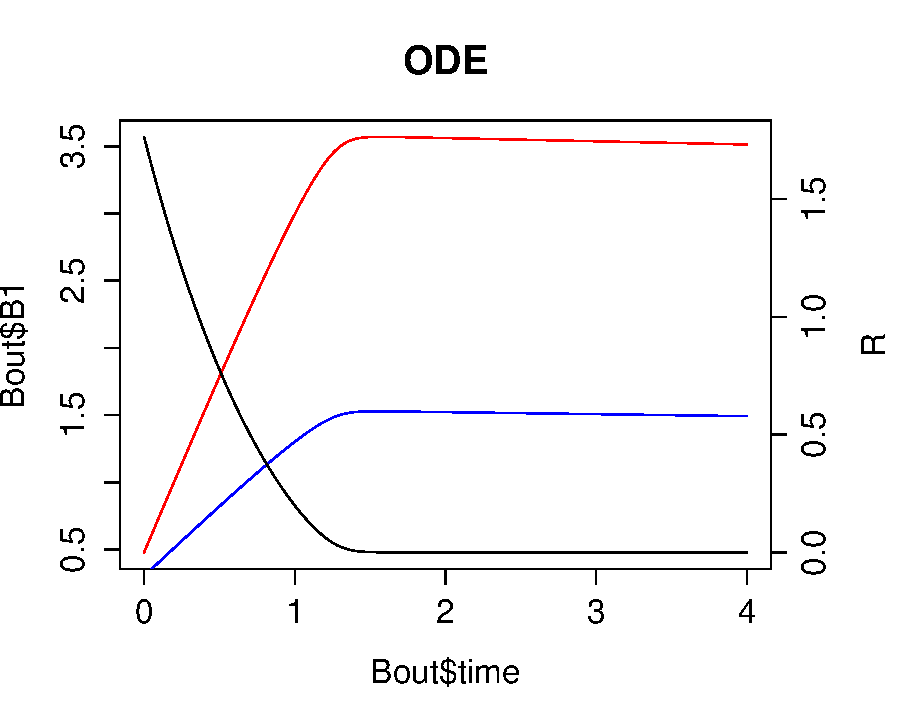
\includegraphics[width=0.8\textwidth]{/20140908_1122am_ODEplot.pdf}
\caption{{\bf Compare ODE and StepStep solutions to our equations}}
\end{figure}

\begin{figure}[h!]
\centering
\noindent 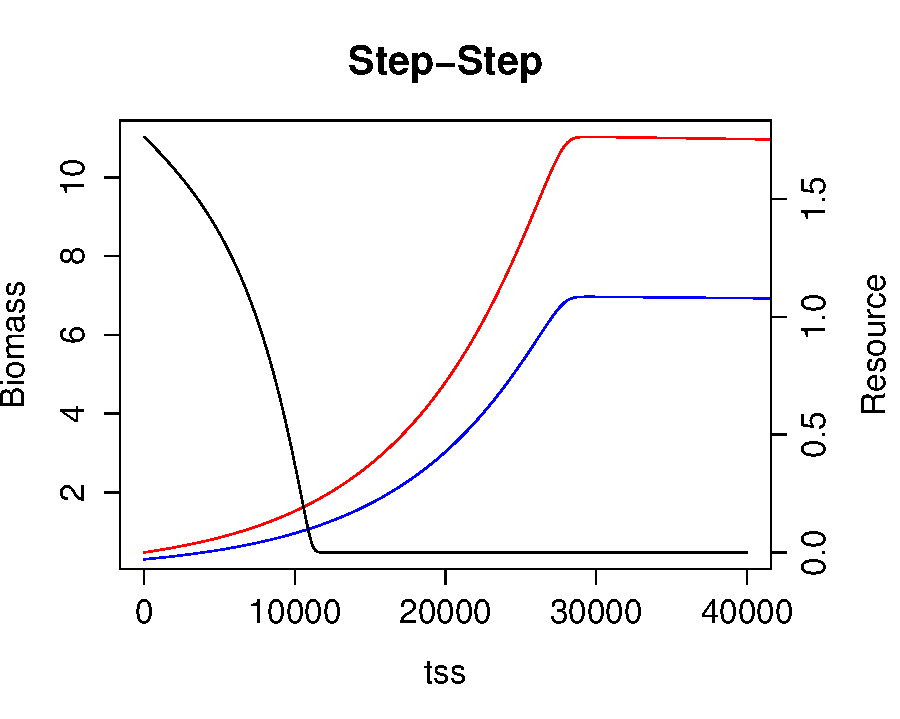
\includegraphics[width=0.8\textwidth]{/20140908_1122am_StepStepPlot.pdf}
\caption{{\bf Compare ODE and StepStep solutions to our equations}}
\end{figure}

\begin{itemize}
\item Step-step solution is clearly incorrect: the resource does not decline exponentially, as it should, and there is no apparent relationship between the decline of resources and the biomass of competing plants
\item The ODE solution appears to be correct.
\item Re-running the Nov 6, 2013 code that Lizzie dug up shows that in that simulation which we thought was working, resources do not decline exponentially.  The Biomasses do stop rising abruptly when R reaches R*, but that is because the loop is forced to end when R < min(R*).  The ODE solution does not end when R<R*.
\item NEXT  STEPS: 
\item solve for long-term equilibrium solution for fixed value of R and g -- where do we expect the equilibrium to be?
\item 
\end{itemize}

\section{Megan: September 22, 2014}
\begin{itemize}
\item Within year dynamics: with the current model runs, the only thing that changes from year to year are the initial conditions.  The equations describing the within year dynamics are exactly the same - including the constants.  The *only* differences are R0 (initial condition for resources) and tauI and tauP, which determine the germination fraction and, therefore, B0 for each species.
\item essentially, create a map showing the end-of-year biomass of species 1 as a function of beginning of year biomass for species 1, beginning of year biomass for sp2, and R0 (this is what the ODE solver does each time)
\item then the question is simply: how do we get a long-run positive average of BiomassOut/BiomassIn for each species?  
\end{itemize}


\section{Megan: September 29, 2014}
\begin{itemize}
\item So, create two 3 dimensional matrix with axes: initial biomass for sp1, initial biomass for sp2, and R0.  Fill one with final biomass for sp 1 and fill the other with final biomass for sp2.
\item Need to figure out how to make ode solver stop when R reaches Rstar.  Runs would be much faster if I could get that to work
\end{itemize}
\begin{figure}[h!]
\centering
\noindent 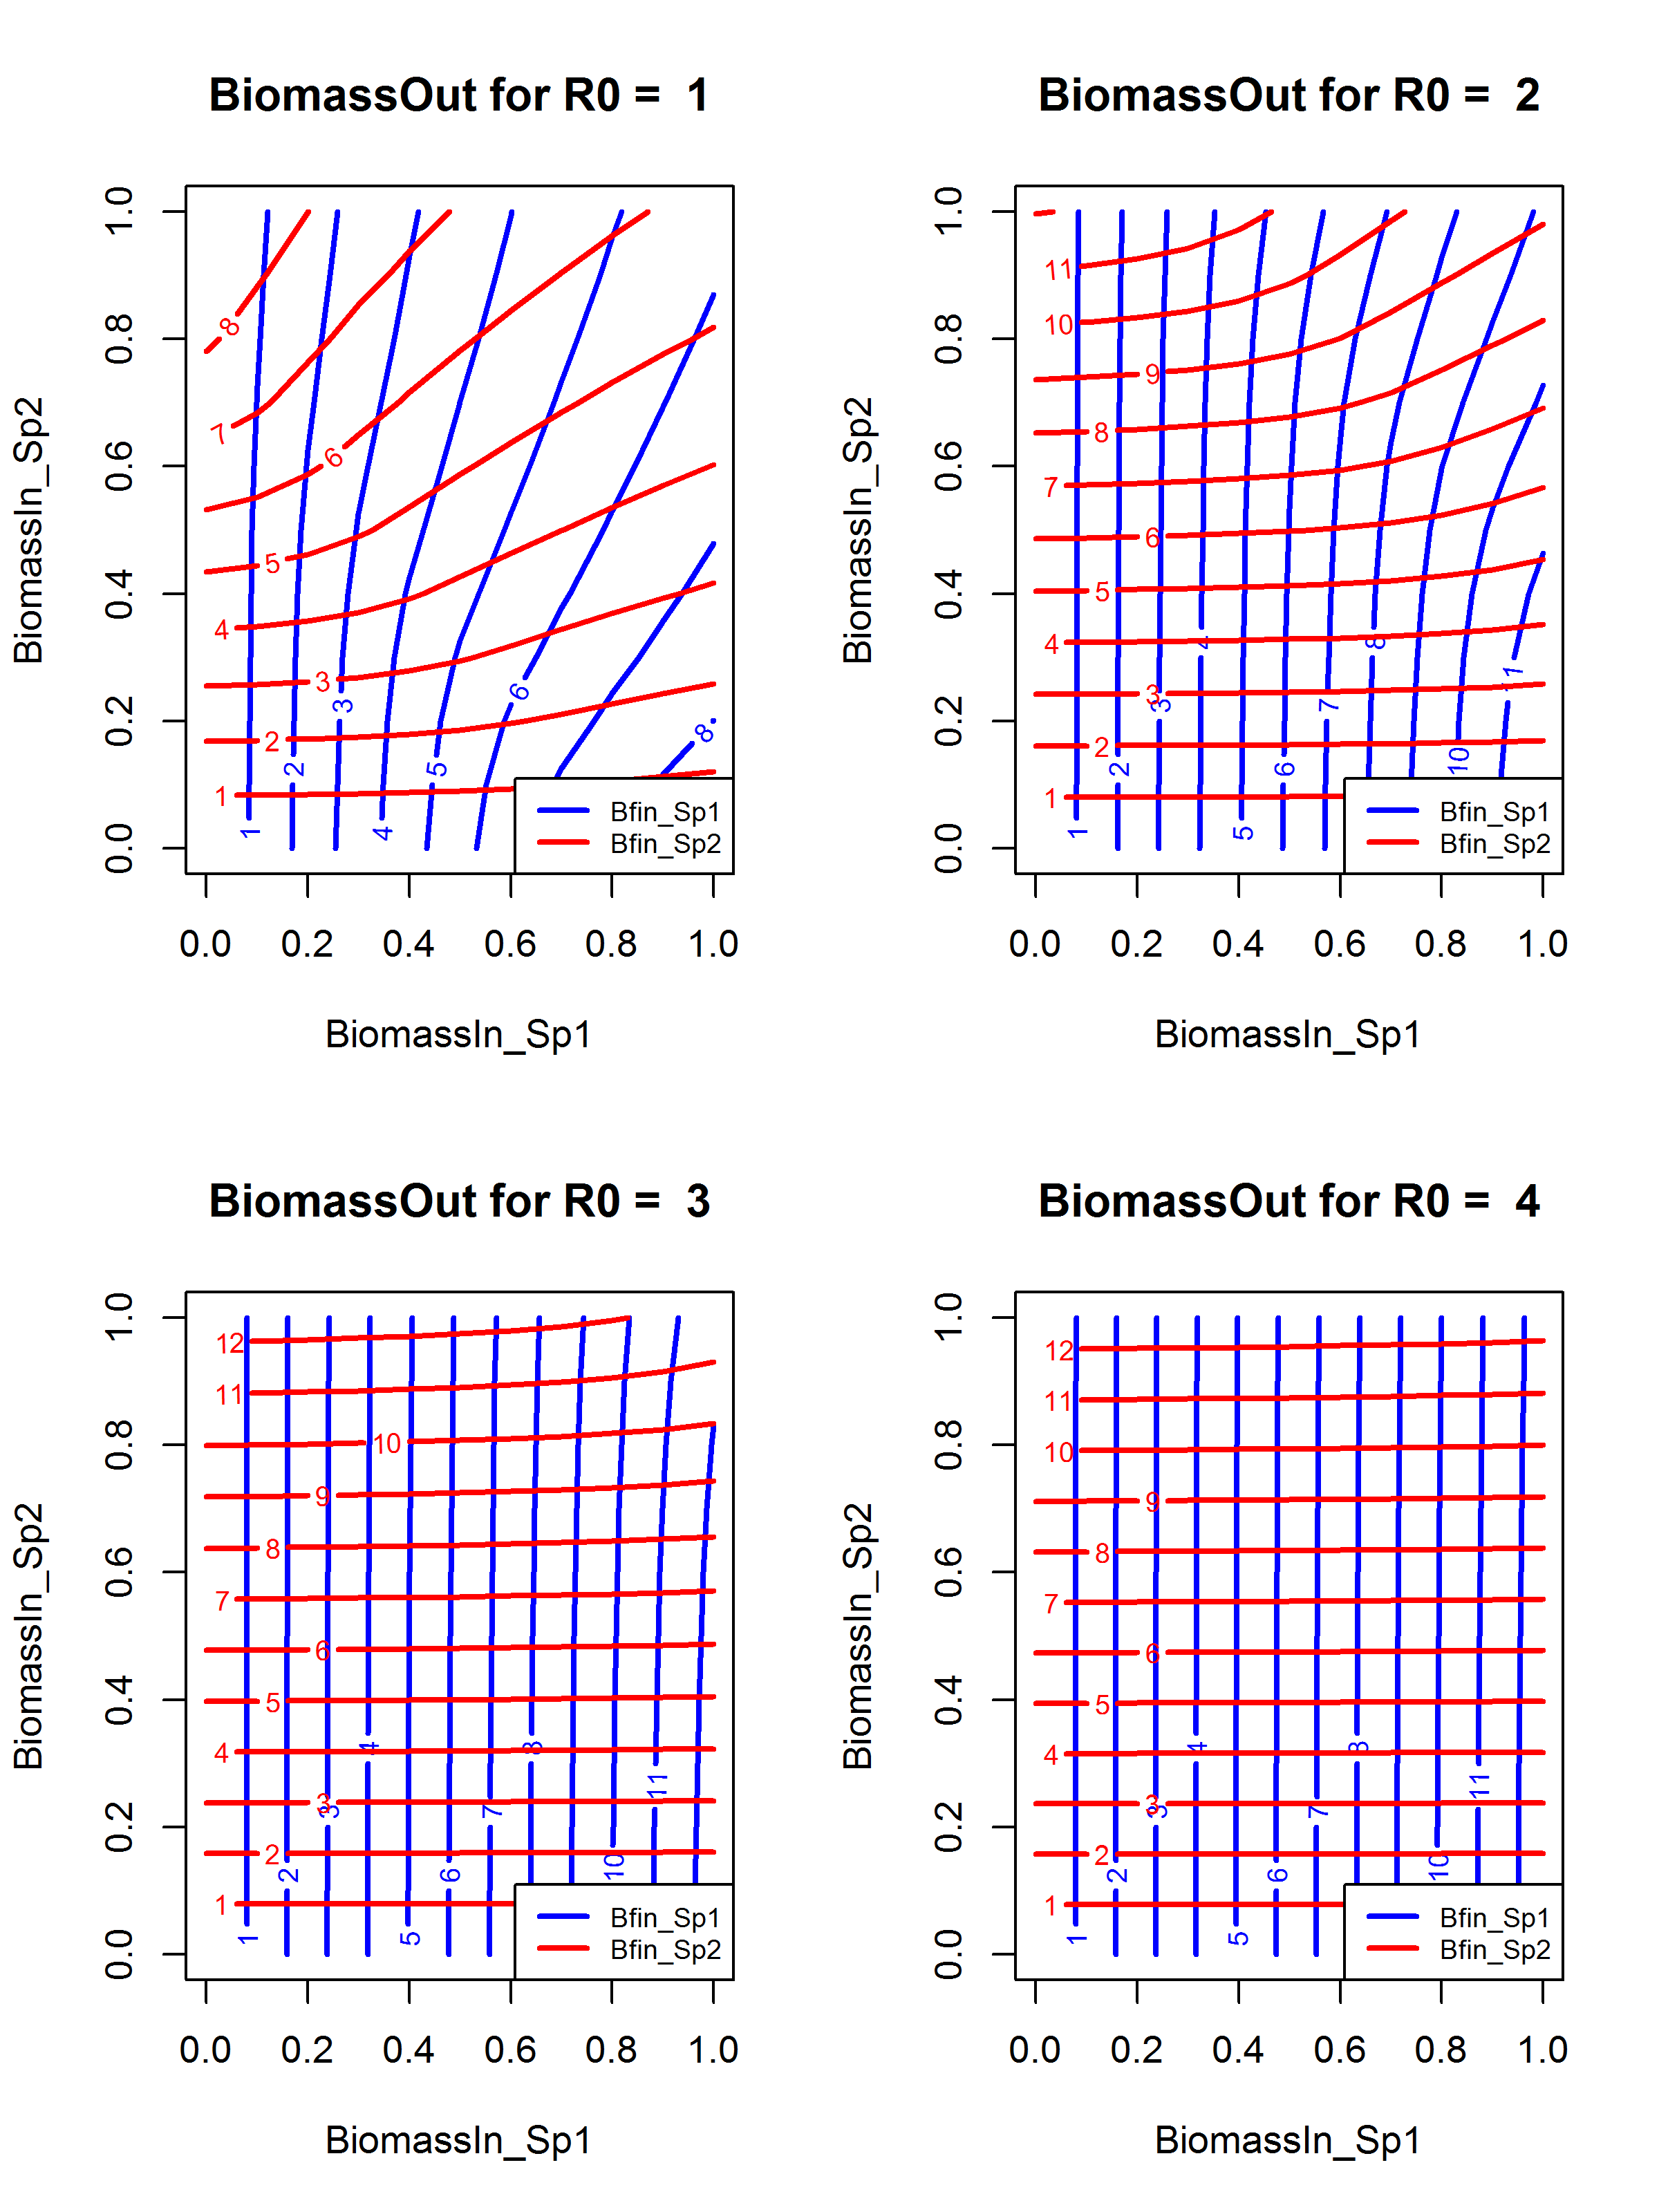
\includegraphics[width=0.8\textwidth]{/WithinYear_BiomassOutvBiomassInvR.png}
\caption{{\bf Contour plots of Biomass Out of Sp 1 (blue) and Sp 2 (Red) for BiomassIn of Sp1 (x-axis) and Sp2 (y-axis) at different levels of R0}}
\end{figure}

\section{Megan & Lizzie meeting: Oct 8, 2014}
\begin{itemize}
\item need to run within year dynamics longer for higher resource levels:  the reason R0=-4 is parallel is because we aren't actually seeing competitive dynamics yet
\item  also plot (Bio1In/Bio1out)/(Bio2In/Bio2Out)
\item figure out how to break ODE solver when R= Rstar
\item does it make sense to convert things to log scale to look at multiplicative rates of increase
\end{itemize}

\end{document}

